\documentclass[a4paper, 12pt]{article}
\usepackage[top=2cm, bottom=2cm,left=2.5cm, right=2.5cm]{geometry}
\usepackage[utf8]{inputenc}
\usepackage{amsmath, amsfonts, amssymb}
\usepackage{float}
\usepackage{graphicx}
\renewcommand*\contentsname{Sum\'ario}
\begin{document}

\title{Trabalho 03 - Programa\c{c}\~ao em linguagem do Montagem MIPS: Aritm\'etica em Ponto Flutuante}
\author{Adailson Pinho dos Santos - 13/0140724\\
Vitor Nere Ara\'ujo Ribeiro - 13/0137413}
\date{}
\maketitle

\newpage

\tableofcontents

\newpage

\section{Introdu\c{c}\~ao}
	\paragraph{}	Este documento tem como objetivo relatar o desenvolvimento do trabalho 3 da mat\'eria Fundamentos de Arquitetura de Software, descreve tamb\'em qual ambiente de desenvolvimento utilizado e quais s\~ao as instru\c{c}\~oes de uso. 
	\paragraph{}	O trabalho 3 consiste em desenvolver um programa em linguagem de montagem Assembly MIPS que realize o c\'alculo do arc-seno de um n\'umero real no intervalo entre -1 e 1. No final podemos exibir o resultador com precisão de 2 casas ou 3, na qual escolhemos por 2 casas de precis\~ao. 
\section{Ambiente de desenvolvimento}
    \paragraph{}	Para a execu\c{c}\~ao do desenvolvimento das aplica\c{c}\~oes foram utilizados os Sistemas Operacionais Fedora 26 e Debian 9, sendo que ambos s\~ao distribui\c{c}\~oes populares do Linux. 
    \paragraph{}	Foi utilizado o simulador de MARS para programar em linguagem de montagem MIPS, a vers\~ao utilizada foi a v4.5 disponibilizada em agosto de 2014, esse software que foi desenvolvido em Java foi essencial para o desenvolvimendo do trabalho. A vers\~ao do Java(TM) SE Runtime Environment utilizado para a execu\c{c}\~ao do simulador MARS foi a v1.8.0.
\section{Constru\c{c}\~ao}
\paragraph{}	A n\'ivel de constru\c{c}\~ao do software a dupla utilizou os procedimentos: \_\_start, \_\_end ler\_real, calc\_arcsen, round e imprime\_saida. No c\'odigo fonte s\~ao descritos os coment\'arios relativos ao funcionamento de cada procedimento e suas rela\c{c}\~oes.
\paragraph{}	A equipe utilizou apenas as seguintes instru\c{c}\~oes: jal, li, syscall, la, mov.s, jr, addi, mtc1, cvt.s.w, mul.s, sub.s, beq, j, cvt.w.s, c.ls.s e bc1f.

\section{Racioc\'inio l\'ogico} 
	\paragraph{}	Na trigonometria, o arcoseno est\'a definido como a funç\~ao inversa do seno.
	\begin{figure}[H]
		\centering
		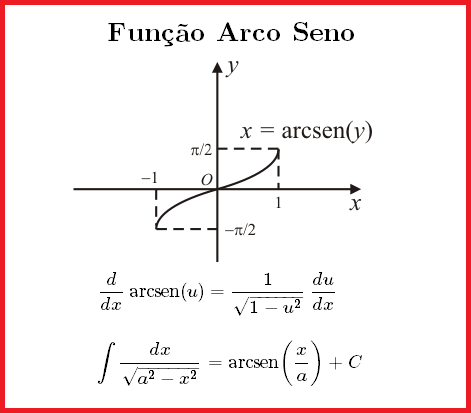
\includegraphics[scale=0.5]{img9.png}
	\end{figure}
	\paragraph{}	S\'erie de Taylor \'e uma s\'erie de pot\'encias infinita. A s\'erie de Taylor para o arcoseno \'e:
	\begin{figure}[H]
		\centering
		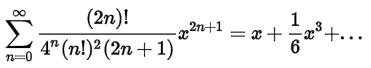
\includegraphics[scale=0.5]{img10.png}
	\end{figure}
        
\section{Instru\c{c}\~ao de uso}
		\paragraph{}    Primeiramente, se deve baixar o MARS Simulator no site do MARS e entrar na pasta onde se encontra o MARS: 
		\begin{figure}[H]
			\centering
			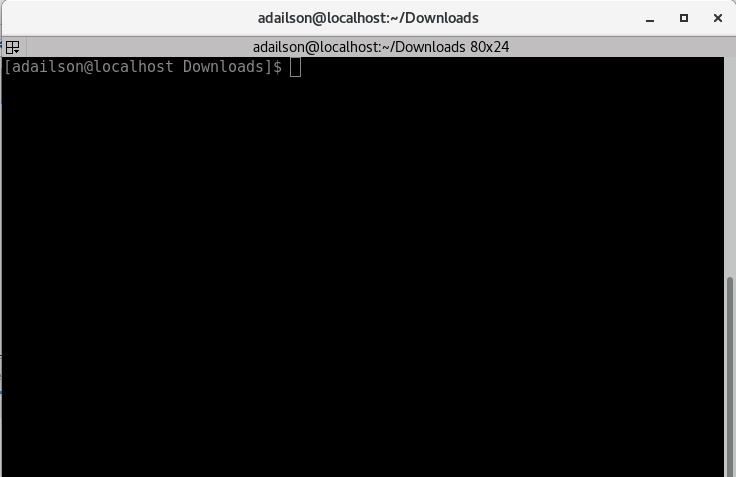
\includegraphics[scale=0.5]{img1.png}
		\end{figure}
		\paragraph{}    Executar o simulador da seguinte forma:
		\begin{figure}[H]
			\centering
			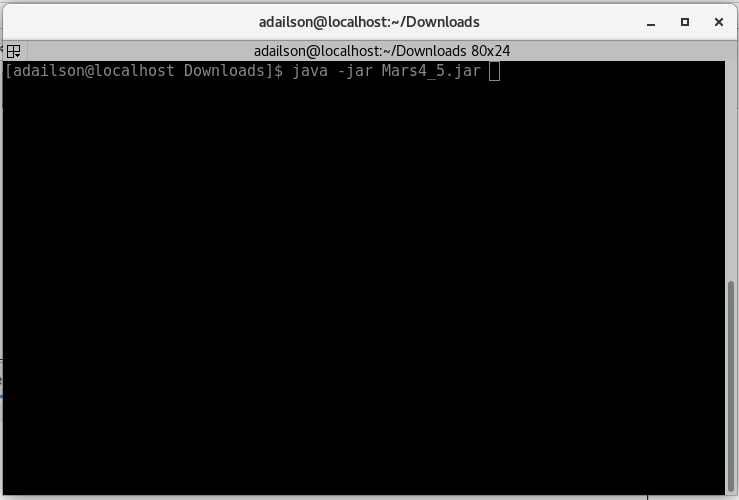
\includegraphics[scale=0.5]{img2.png}
		\end{figure}
        \paragraph{}    Com o MARS simulator aberto, o usu\'ario deve abrir o arquivo .ASM que cont\'em as instru\c{c}\~oes em Assembly MIPS:
        \begin{figure}[H]
        	\centering
        	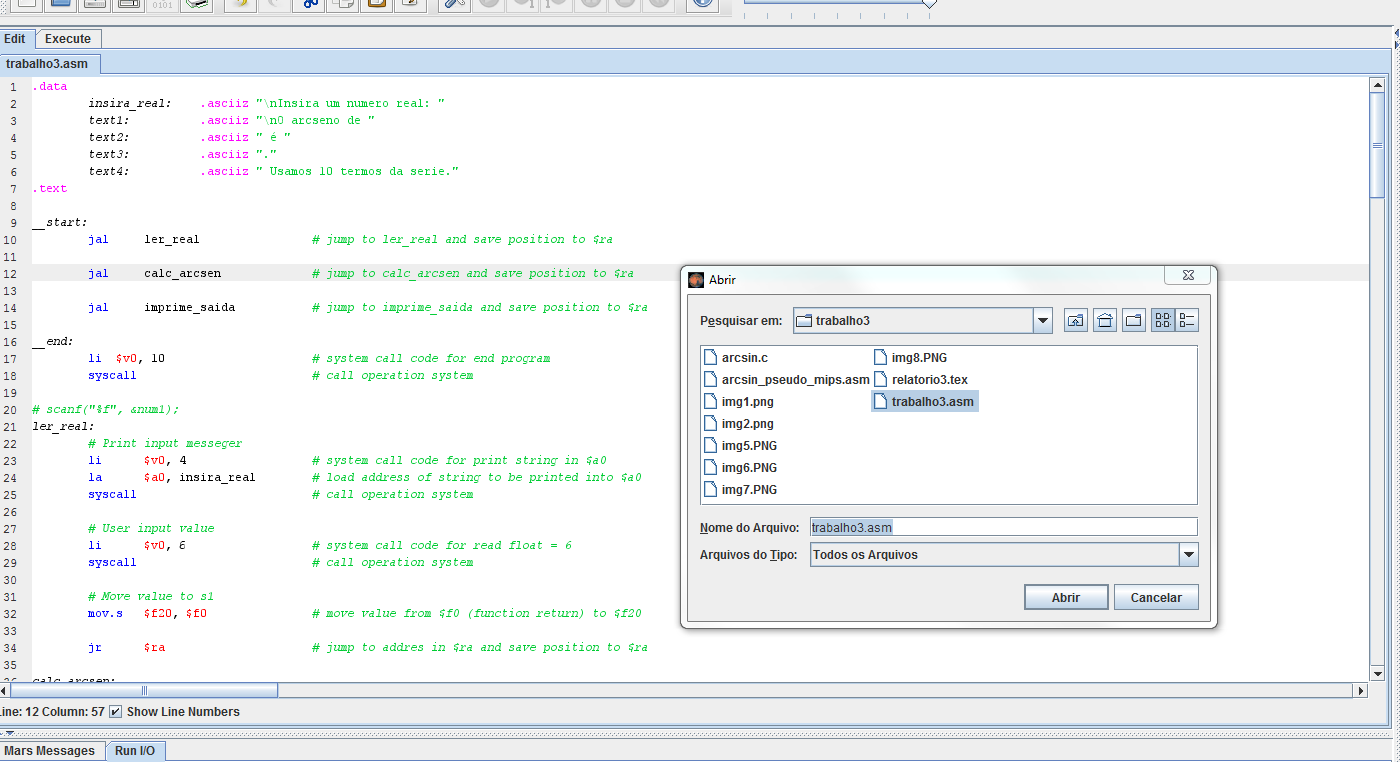
\includegraphics[scale=0.5]{img3.png}
        \end{figure}
        \paragraph{}    Primeiro caso de teste, o usu\'ario deve clicar na Aba Run-Assemble para montar o programa e Run-Go para executar o programa. Inserir o valor 1 ou 1.0, a resposta deve consistir em: "O arcseno de 1.0 \'e 1.57. Usamos 10 termos da serie.":
        \begin{figure}[H]
        	\centering
        	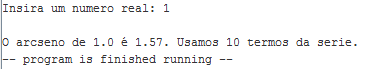
\includegraphics[scale=0.8]{img5.png}
        \end{figure}
        \paragraph{}    No segundo caso de teste, \'e inserido o valor de -1, A resposta deve consistir: "O arcseno de -1.0 \'e -1.57. Usamos 10 termos da serie.":
        \begin{figure}[H]
        	\centering
        	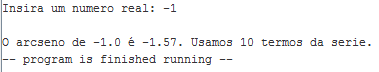
\includegraphics[scale=0.8]{img6.png}
		\end{figure}
		\paragraph{}     No terceiro caso de teste, \'e inserido o valor de 0.866, A resposta deve consistir: "O arcseno de 0.866 \'e 1.05. Usamos 10 termos da serie.":
        \begin{figure}[H]
        	\centering
        	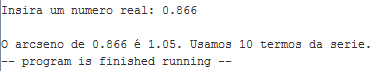
\includegraphics[scale=0.8]{img7.png}
        \end{figure}
        \paragraph{}    No quarto caso de teste, \'e inserido o valor de -0.866, A resposta deve consistir: "O arcseno de -0.866 \'e -1.05. Usamos 10 termos da serie.":
        \begin{figure}[H]
        	\centering
        	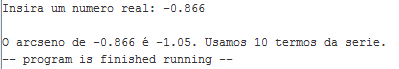
\includegraphics[scale=0.8]{img8.png}
		\end{figure}
		
        \paragraph{}    
\end{document}
